\begin{itemize}

\item The increasing severity of the effects of climate change, especially strengthening extreme events and wildfire, is theatening built infrastructure, utilities, and national and economic security.

\item Loss of life and property is motivating serious consideration of approaches for \textbf{climate intervention} or \textbf{geoengineering}.

\item In addition to efforts to scale up \textbf{carbon dioxide removal (CDR)} through \textbf{direct air capture (DAC)} and other means, interest in growing in methods to reduce or stabilize Earth's surface temperature.

\item \textbf{Solar radiation management (SRM)} is one approach to partially reduce warming by reflecting a portion of incoming solar radiation to maintain resilience of the Earth system.

\item \textbf{Stratospheric aerosol intervention (SAI)}, through direct injection of sulfur into the lower stratosphere, is considered the most feasible scheme.

\item Many questions remain unanswered regarding the feedback effects of SAI on the Earth system.

\end{itemize}

\begin{figure}
	\begin{center}
		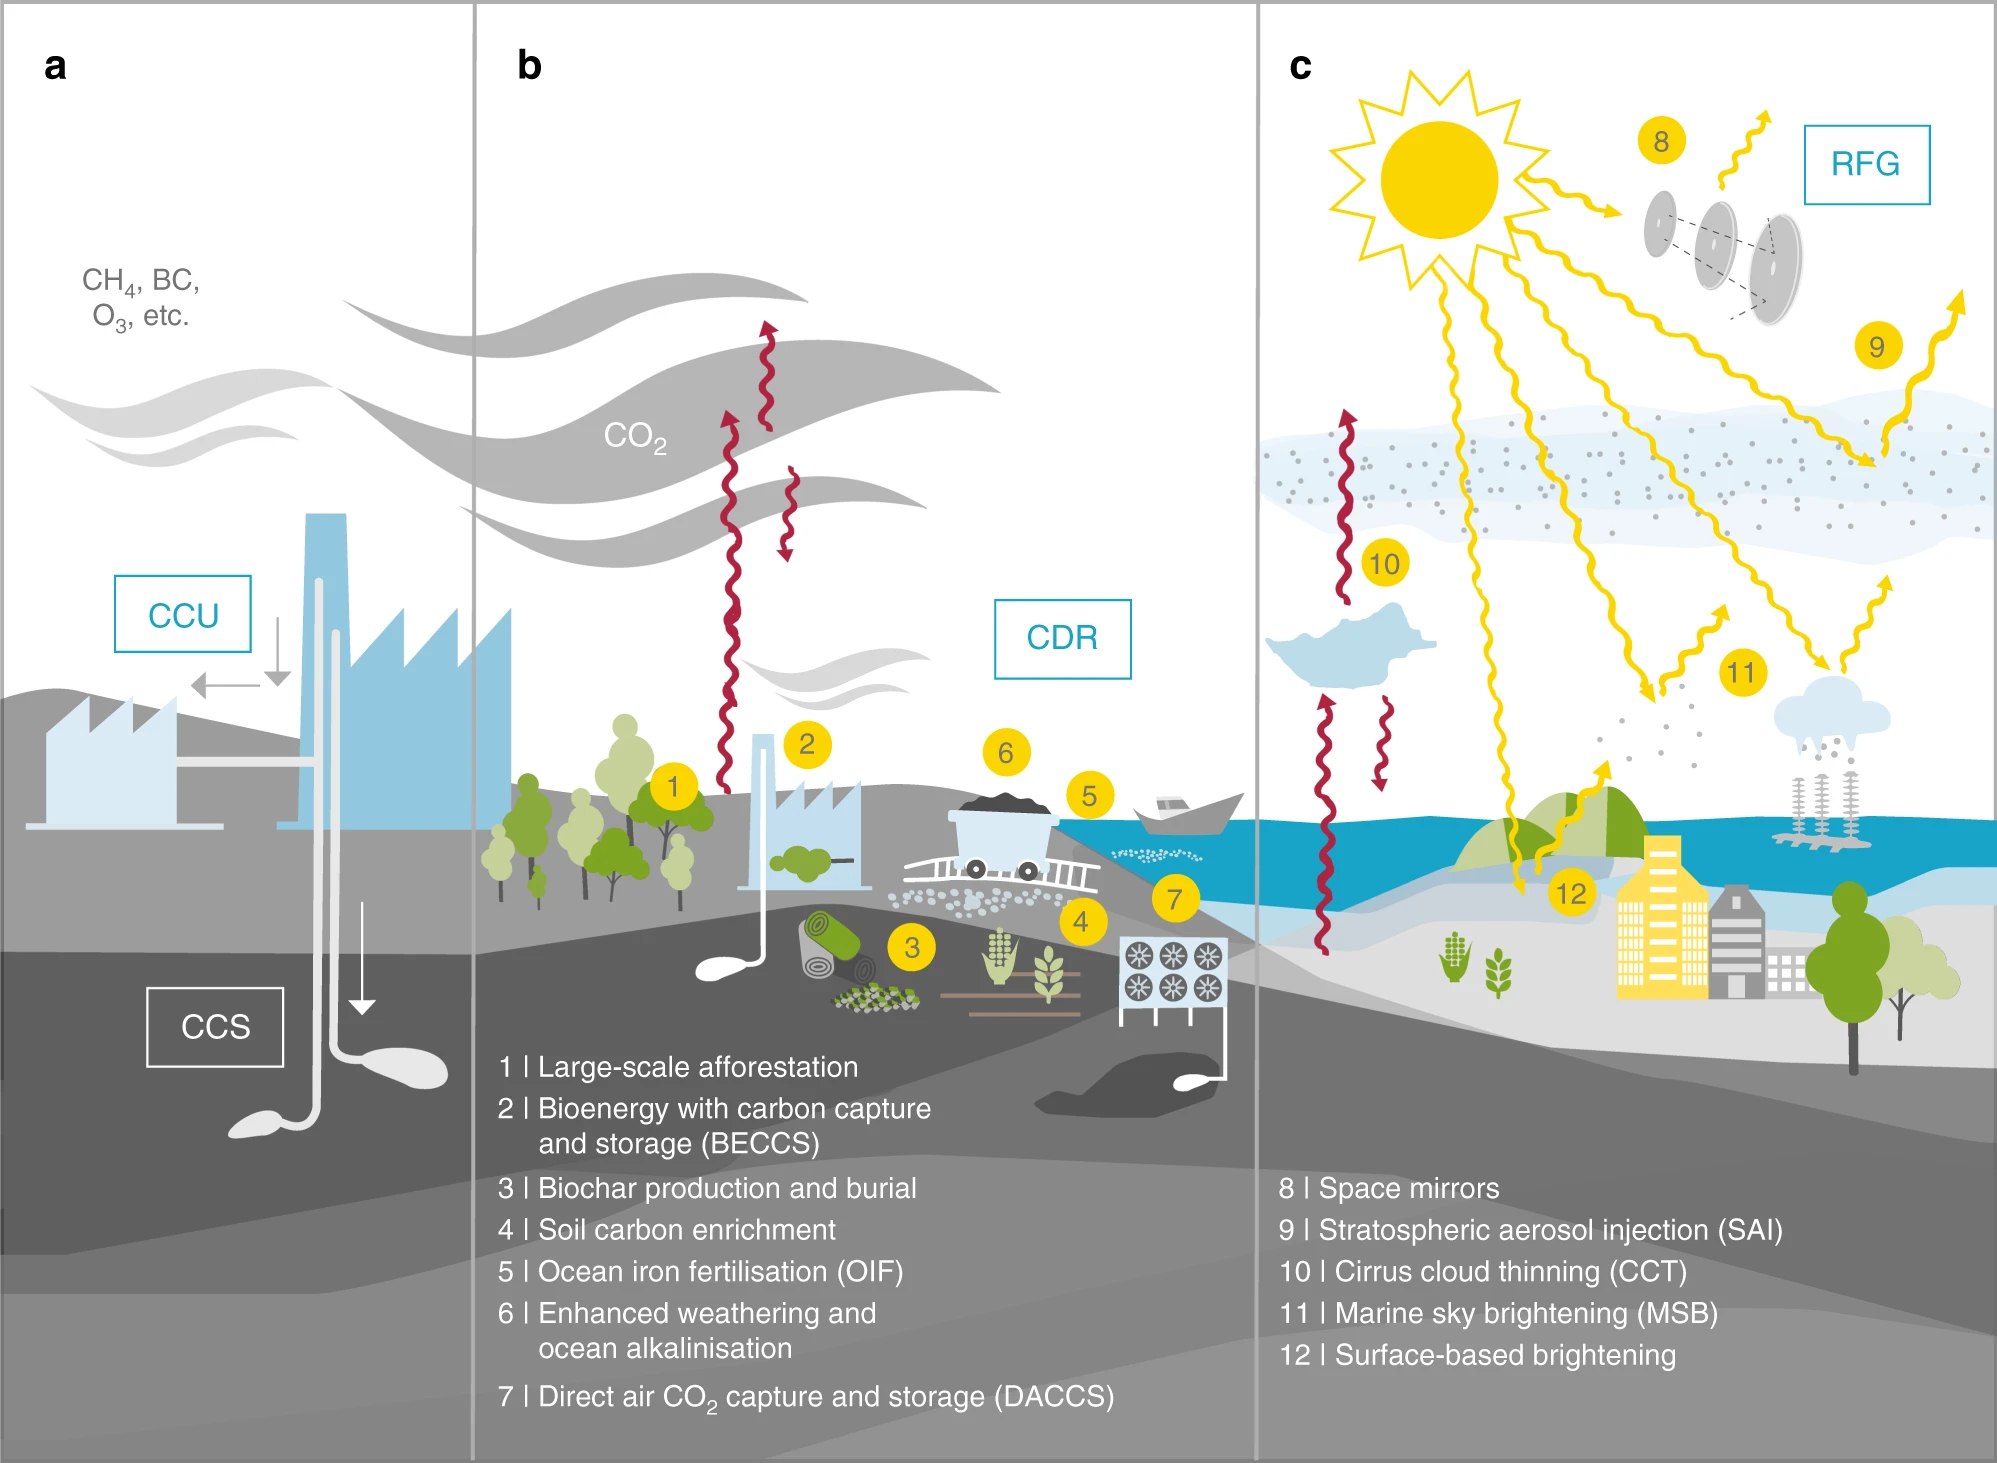
\includegraphics[width=0.8\columnwidth]{figures/41467_2018_5938_Fig1_HTML.png}
	\end{center}
	\caption{Proposed climate geoengineering techniques placed in the context of mitigation efforts. Adopted from Lawrence et al. (2018).
		% https://www.nature.com/articles/s41467-018-05938-3
	}
\end{figure}
